
\chapter{Background and Context}


\section*{Introduction}

In this chapter, we start by presenting Mohammed VI Polytechnic University (UM6P) as a leading institution in the advancement of research, innovation, and development in Africa. Ai movement is a research-based centre affiliated with the UM6P group and which aspires to be the African leader in artificial intelligence. This center is dedicated to growing Moroccan and African talent in AI and Data Sciences, solving complex problems with innovative, ethical, and scalable solutions, and building the next generation of leaders in this field. In this post, we are going to go through a variety of programs and initiatives run by Ai movement and talk about how Ai movement is driving the change in AI landscapes everywhere.
The second part of this chapter then outlines the specific framework of our project. We introduce the real-world context of multi-agent coordination, particularly for Unmanned Aerial Vehicles (UAVs) operating in partially observable environments. Finally, we define the core objectives of this work, which are centered on developing a novel, learning-informed masking strategy to enhance multi-agent reinforcement learning performance under these challenging conditions.

\section{Presentation of the Host Organization}

The following sections introduce UM6P and the main contributions to artificial intelligence from the Ai movement center. As stated by Pr. Ai movement Executive President, Amal El Fallah Seghrouchni: "Within Mohammed VI Polytechnic University, we have created the Moroccan International Center of Artificial Intelligence called the Ai movement. In order to accompany the transformations induced by the advent of Artificial Intelligence and Data Sciences, to promote the emergence of a Moroccan and African know-how, and to meet the many challenges raised by AI. Whether they are scientific, technological, or ethical, our center promotes a hybrid and integrative approach to build deep AI and full stack of AI systems taking advantage of the complementarity of different AI paradigms." 


\begin{figure}[H]
  \centering
  
\includegraphics[width=0.75\textwidth]{images_pfe/AIM-UNESCO_EN.png}
  \caption{Logo Ai movement.}
\end{figure}
\FloatBarrier



\subsection{Mohammed VI Polytechnic University}

Mohammed VI Polytechnic University (UM6P), known in French as Université Mohammed VI Polytechnique, is a non-profit private research university in Morocco. Its main campus is located in the Green City of Benguerir. Focused on African development, the university prioritizes applied research and innovation, contributing to regional economic and human development. 

UM6P is a dynamic institution that fosters interdisciplinary collaboration and transformative learning experiences. It nurtures competent leaders with social responsibility and a passion for change in diverse fields. As a hub for experimentation, it empowers lifelong learners through innovative pedagogy and inclusive environments. UM6P's research initiatives drive economic and human development in Africa, forging global partnerships and promoting excellence, social responsibility, and sustainable development. Its missions include developing competent leaders, promoting research, fostering collaboration, empowering students and communities, and advancing African development, embodying a commitment to excellence, innovation, and positive change.

\begin{figure}[hbt!]
  \centering
  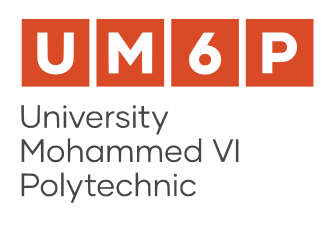
\includegraphics[width=0.3\textwidth]{images_pfe/um6p_logo.png}
  \caption{Logo Mohammed VI Polytechnic University.}
  \label{fig: Fusion PSA et FCA}
\end{figure}
\FloatBarrier



UM6P welcomed its first students in 2013 and was officially inaugurated on January 11, 2017. Since then, it has grown into a leading research institution, facilitating collaborations between Africa and Europe. The university is home to the most powerful supercomputer in Africa and encompasses several schools and research institutes, some of which existed before the university was established. UM6P maintains numerous international partnerships with prestigious institutions such as the Massachusetts Institute of Technology, Columbia Business School, Max Planck Society, HEC Paris, Mines ParisTech, the École Polytechnique Fédérale de Lausanne, McGill University, and Sciences Po.


UM6P was established as part of the major urban development projects initiated by His Majesty King Mohammed VI of Morocco. It symbolizes Morocco's commitment to education, research, and innovation as drivers of national and regional progress. The university's creation reflects King Mohammed VI's vision to promote higher education and the knowledge economy in Morocco, emphasizing excellence and sustainability.

The university has continuously expanded its reach, attracting students and scholars from across the continent and around the world. Its mission is to promote research, innovation, and sustainable development, addressing the pressing challenges facing Africa. Currently, UM6P hosts 5,684 students from over 20 nationalities, predominantly from sub-Saharan Africa, and has partnerships with universities across Africa, Europe, Asia, and the Americas.



Committed to excellence in education, research, and innovation, UM6P focuses on advancing Africa's development in various domains, among its faculties: 
\begin{itemize}
    \item Africa Institute for Research in Economics and Social Sciences
    \item Public Policy School
    \item The Faculty of Governance, Economics and Social Sciences
    \item School of Agriculture, Fertilization and Environmental Sciences
    \item School of Architecture, Planning and Design, Africa Business School
    \item School of Collective Intelligence
    \item School of Hospitality Business $\&$ Management
    \item Institute of Science, Technology $\&$ innovation


\end{itemize}


Its key missions encompass developing competent leaders through interdisciplinary learning experiences, promoting applied research to address societal challenges, instilling values of social responsibility and sustainable development, fostering collaboration with global partners, empowering students and communities to enact positive change, and advancing Africa's development through research, education, and innovation initiatives. Through these multifaceted missions, UM6P serves as a catalyst for positive change and transformation, shaping the future of Africa and inspiring the next generation of leaders and innovators.



\subsection{Ai movement Center}

Ai movement, Morocco's International Center for Artificial Intelligence, is a center of excellence dedicated to fostering Moroccan expertise in AI and Data Sciences. It serves as both:
\begin{itemize}
    \item A \textbf{coordinating and consolidating platform} for various AI-related initiatives, with the goal of establishing Morocco as a regional AI hub impacting strategic, educational, and industrial ecosystems.
    \item A \textbf{proactive force} to anticipate and guide the transformations associated with AI and Data Sciences, aiming to deliver innovative, practical, resilient, and ethical solutions to societal, environmental, market, economic, and technological challenges.

\end{itemize}


Ai movement, located at Mohammed VI Polytechnic University in Rabat, strives to advance Moroccan and African expertise in artificial intelligence (AI) and data sciences. As the first \textbf{UNESCO category 2 AI center in Africa}, it aims to make Morocco a regional AI hub that influences strategic, educational, and industrial sectors.

The center advocates for the development of ethical and responsible AI to enhance social welfare ("AI for Good") and promotes a creative economy by empowering youth with the skills needed to drive innovation. Its mission includes building an inclusive knowledge society by democratizing access to AI and data sciences while ensuring privacy and data protection.

Research efforts at the center focus on both theoretical and practical advancements, aimed at developing impactful and reliable technological solutions for various sectors, from agriculture to aerospace. The center fosters innovation and creativity, generating products designed to meet contemporary societal needs.

At the core of the center are its talented researchers and experts, specializing in diverse AI areas such as machine learning, computer vision, and robotics. Equipped with cutting-edge infrastructure and ample computing resources, the center provides an ideal environment for research and development.


\subsection{History of um6p}
The university was established as part of the "Green City" project, a significant urban development initiative located just outside the historic city of Ben Guerir. The project's goal is to create a model city of sustainability, with a special emphasis on promoting research, education, and development in Africa. The construction of the university began in 2012, and it started operating in 2013. Over the years, numerous schools and research centers were founded or integrated into the university.

In 2021, UM6P launched Africa's most powerful supercomputer for scientific research and innovation. The African Supercomputing Center, with a capacity of 3.15 petaflops capable of performing three million billion operations per second, provides Morocco and the broader African continent with significant opportunities to advance in scientific research and innovation across various fields.
\subsection{Ai movement OCP UNESCO}

\subsubsection{Ai movement-UM6P Receives UNESCO Category II Status}
The Ai movement-UM6P in Morocco has been granted UNESCO Category II status, marking it as the first Category II center for artificial intelligence in Africa. UNESCO's Category II centers serve as international or regional hubs of expertise, providing technical assistance and services to member states, cooperation partners, and UNESCO's decentralized network.

This designation underscores Morocco's regional leadership in emerging technologies, particularly in the field of artificial intelligence, and reaffirms its commitment to the ethical principles of AI. The Permanent Delegation of Morocco to UNESCO has welcomed this decision, emphasizing its potential to boost regional and multilateral cooperation in AI, thereby fostering economic growth and social development across Africa.



\subsubsection{OCP and Ai movement Partnership}
Founded in 2021 by OCP, the Moroccan Center for Artificial Intelligence, known as Ai movement, represents the fertilizer giant's primary investment in this technological revolution. As Morocco works towards developing a dedicated AI action plan, this project stands as a pioneering effort. Demonstrating OCP's ambition, the center, which has received significant investment in education and energy transition, hosts the famous \textbf{African AI summit} annually.
% \vspace*{0.2cm}

% \begin{figure}[hbt!]
%   \centering
%   
\includegraphics[width=0.68\textwidth]{images_pfe/Screenshot from 2024-06-09 20-05-22.png}
%   \caption{Aim supported by OCP group, designated as he first Category II center of AI in Africa by UNESCO}
% \end{figure}
% \FloatBarrier

\subsection{Technical data of Ai movement}


\definecolor{lightblue}{rgb}{0.78, 0.85, 0.92} % lighter shade of blue
\begin{table}[!ht]
\centering
\renewcommand{\arraystretch}{1.4} % row height spacing
\setlength{\tabcolsep}{8pt}       % column padding
\begin{tabular}{|>{\columncolor{lightblue}}m{4cm}|m{10.4cm}|}
\hline
\textbf{Center Name} & Ai movement \\
\hline
\textbf{Date of Establishment} & 11th November, 2022 \\
\hline
\textbf{Headquarters} & Rabat, Morocco \\
\hline
\textbf{Management} & CEO: Pr. Amal El Fallah Seghrouchni \\
\hline
\textbf{Products} & Artificial Intelligence solutions and Innovative software and 
algorithms for data analysis, machine learning, and predictive modeling. \\
\hline
\end{tabular}
\caption{Technical data of Ai movement}
\label{tab:ai_movement_techdata}
\end{table}

\FloatBarrier

\subsection{Mission of Ai movement}

The mission and research focus of UM6P is deeply committed to advancing research, fostering innovation, and promoting development across Africa. It collaborates with numerous institutions in African countries, establishing experimental research platforms and applied research laboratories in partnership with universities across the continent. One of UM6P's prominent research laboratories is MSDA, which stands for Modeling, Simulation, and Data Analysis. This lab specializes in mathematical and phenomenological modeling, numerical simulation, and data analysis.

The Ai movement serves as a coordinating and consolidating tool for various AI-related initiatives, aiming to establish Morocco as a regional AI hub impacting its ecosystem on strategic, educational, and industrial levels. It is designed to anticipate and support the evolution and transformation related to Artificial Intelligence and Data Sciences, providing innovative, operational, resilient, and ethical solutions to societal, environmental, market, economic, and technological challenges.

The program aims to prepare leaders to responsibly drive artificial intelligence projects through a comprehensive portfolio of units covering key AI technologies, managerial tools for driving technological change, and business-oriented use cases. The \textbf{program's objectives} include:
\begin{itemize}
    \item Understanding different AI techniques and familiarizing with industry-specific terminology.
    \item Exploring advanced machine learning architectures with a focus on applications in computer vision, language processing, cybersecurity, and robotics.
    \item Harnessing AI techniques for informed adoption in business processes.
    \item Acquiring governance skills for leaders, covering trusted AI, data management, regulation, and ethics.
\end{itemize}
\begin{figure}[H]
  \centering
  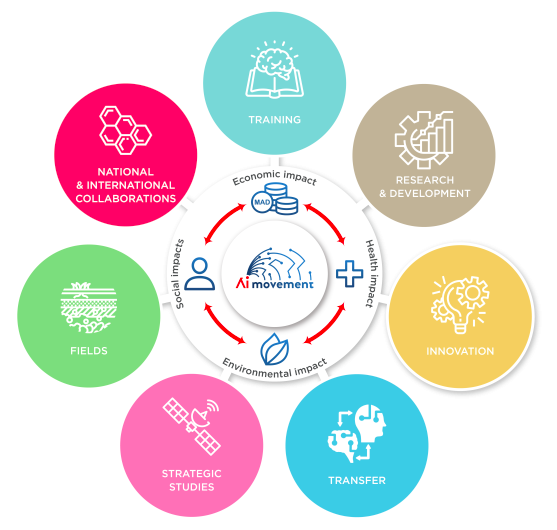
\includegraphics[width=0.3\textwidth]{images_pfe/Screenshot from 2024-06-08 18-57-32.png}
  \caption{Pillars of Ai movement.}
\end{figure}
\FloatBarrier

Structured around several pillars, the \textbf{Ai movement's initiatives} aim to:

\begin{enumerate}
    \item Develop an attractive ecosystem by fostering international collaborations and nurturing local talent.
    \item Advocate for a field-oriented approach to drive societal acceptance and understanding of AI transformations.
    \item Offer inclusive training programs tailored to various age groups and skill levels.
    \item Integrate theoretical research with practical applications to facilitate innovation and industrial transfer.
    \item Conduct strategic studies to anticipate and manage the geopolitical implications of AI advancements.

\end{enumerate}




 \section{Program Offerings}

The Ai movement offers a range of programs tailored to different aspects of artificial intelligence. A central component of our academic offerings is the \textbf{Executive Master in AI Governance and Practice}. This program is composed of the following four stackable certificates, which can be taken individually to gain specific skills or completed together to earn the full Master's degree:

\begin{itemize}
    \item \textbf{C1: AI Foundations Certificate}: Gain knowledge about AI foundations and explore the potential of machine learning in various fields.
    \item \textbf{C2: AI Application Certificate}: Explore the full potential of specific AI architectures for multiple industry applications to develop a strategic understanding of AI.
    \item \textbf{C3: AI Governance Certificate}: Learn about the latest regulations in AI and data management, as well as best practices for responsible and ethical AI.
    \item \textbf{C4: AI Transformation Certificate}: Acquire skills to manage complex AI projects and lead successful AI transformations within organizations.
\end{itemize}

In addition to the Executive Master, the Ai movement is dedicated to fostering inclusivity and early education through two flagship initiatives:

\begin{itemize}
    \item \textbf{African Women in Tech and AI Program}: This initiative supports African women in technological innovation and artificial intelligence, aligning with UNESCO's Operational Strategy for Priority Africa 2022-2029. It empowers cohorts of women to develop and lead impactful projects.
    \item \textbf{AI Master Junior Program:} An exciting initiative designed for children aged 10 to 14, this program introduces the world of AI through interactive, hands-on activities that explore its applications in daily life.
\end{itemize}


\section{Project Framework}

Multi-agent systems composed of UAVs and Unmanned Ground Vehicles (UGVs) are becoming increasingly relevant for real-world tasks such as surveillance, search and rescue, and environment monitoring. However, these agents often operate in GPS-denied or visually occluded environments that restrict their ability to observe the full state of the environment. This project explores how to improve agent coordination and decision-making in such partially observable settings using a \textbf{Masked Auto-Encoder (MAE)}.

Inspired by the effectiveness of MAEs in computer vision and NLP, this work integrates a transformer-based MAE within a Multi-Agent Reinforcement Learning (MARL) framework. The MAE reconstructs masked portions of the input, enabling agents to infer missing environmental features and form richer internal state representations.

The project is built on benchmark environments such as SMAC and SMACv2, simulating complex interactions among multiple agents. Several smart masking strategies are investigated, including random masking and TD-error-based masking. The resulting architecture is evaluated for its ability to enhance sample efficiency, coordination, and task performance.



\subsection{Context: Drone Coordination in Partially Observable Environments}
In GPS-denied or sensor-limited environments such as underground tunnels, forests, and urban disaster zones, UAVs must rely on onboard sensors like LiDAR, RGB cameras, and IMUs. These sensors can fail or provide noisy data, leading to partial observability. Swarms of UAVs must coordinate using local observations while maintaining situational awareness and achieving global objectives.

This research addresses the challenge by enabling each agent to learn latent representations that fill in missing inputs through an MAE trained in a self-supervised manner. These enhanced representations help agents to:
\begin{itemize}
\item Improve local and global awareness despite limited perception.
\item Maintain decentralized coordination in the absence of centralized communication.
\item Make informed decisions with incomplete or corrupted input.
\end{itemize}
\subsection{Objectives of the Project}
This internship project aims to achieve the following goals:
\begin{itemize}
\item Design and implement a masked auto-encoder module that can be integrated with popular MARL algorithms.
\item Explore the impact of different masking strategies (random, TD-error) on training performance.
\item Evaluate the framework in partially observable MARL benchmarks like SMAC and SMACv2.
\item Propose a masking strategy that adapts to agent learning difficulty and environmental complexity.
\item Demonstrate the benefits of the approach through ablation studies and performance comparison with baseline methods.
\end{itemize}

\subsection{Use Case Scenarios }
The project is grounded in real-world inspired scenarios where MARL agents must operate with limited or unreliable perception. The following are the primary use cases guiding this research:

\begin{itemize}
\item \textbf{GPS-Denied Navigation:} In scenarios where GPS is blocked or jammed (e.g., tunnels, urban warfare zones, or indoor operations), drones must rely solely on onboard sensors like LiDAR, RGB cameras, IMUs, and stereo cameras. The AI-based sensor fusion, enhanced by MAE, allows agents to infer location and environmental structure despite missing data.
\item \textbf{Disaster Response:} During post-disaster search and rescue operations, communication may be unstable or absent. UAVs and UGVs deployed in swarms can collaborate to explore hazardous zones, map the terrain, and locate survivors. MAE-enhanced agents help in real-time decision-making based on partial views.
\item \textbf{Autonomous Agriculture:} Swarms of drones can monitor crop health or perform coordinated tasks like pesticide dispersion or harvesting, even when individual sensors fail or encounter occlusions due to vegetation. MAEs help reconstruct consistent representations for collective task execution.
\item \textbf{Military Reconnaissance:} In hostile terrain, drone swarms can perform cooperative surveillance without relying on central control or full visibility. The masked encoding framework improves the agents' ability to maintain situational awareness even when some drones are lost or obstructed.
\item \textbf{Collaborative Exploration and Mapping:} UAV-UGV hybrid swarms can be deployed for 3D terrain reconstruction. While UAVs provide a top-down perspective, UGVs can access and report from ground level. MAEs facilitate alignment of partial, heterogeneous views into unified maps.
\end{itemize}

\subsection{Project Timeline and Work Plan}

To effectively manage the scope of this project, a structured work plan was developed, spanning a six-month period. The timeline, illustrated by the Gantt chart in Figure~\ref{fig:gantt}, outlines the major phases of the research and development process. The project began with a foundational learning period dedicated to reinforcement learning principles, followed by a thorough review of the project context and the state-of-the-art. Subsequent months were allocated to the technical implementation, beginning with the baseline setup and followed by the development of our core contribution, the LI-MA2E framework. The final two months were dedicated to intensive training, evaluation, results analysis, and the final documentation and writing of this thesis.

\begin{figure}[H]
    \centering
    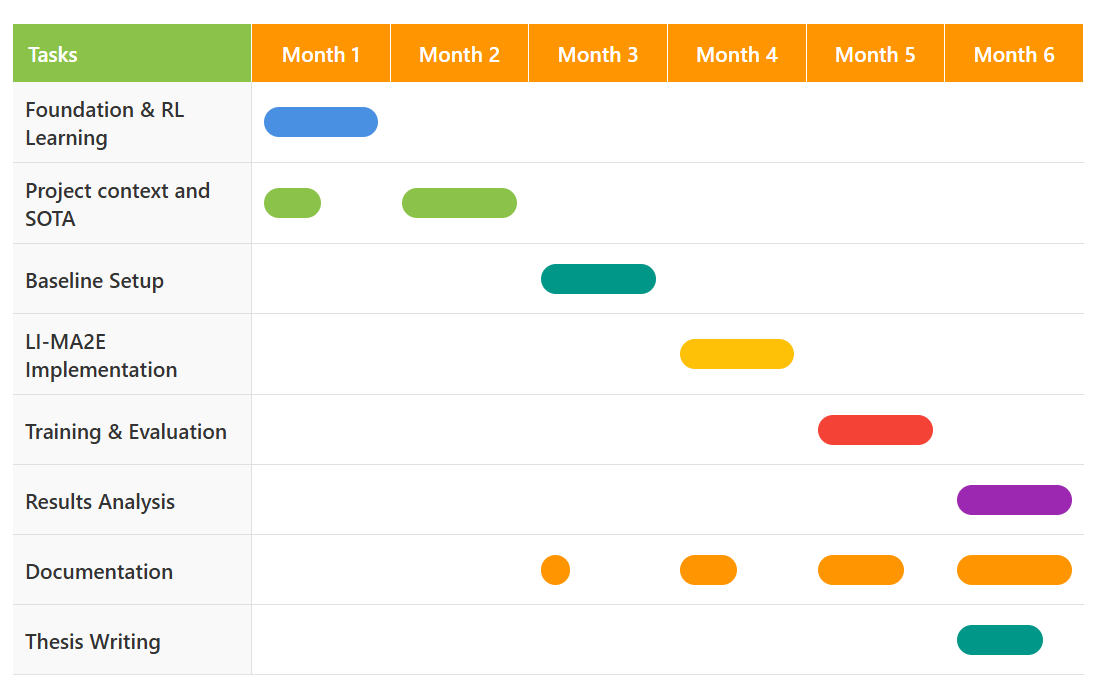
\includegraphics[width=0.7\textwidth]{images_pfe/gant.png}
    \caption{Gantt chart illustrating the project timeline and the distribution of key tasks over a six-month period.}
    \label{fig:gantt}
\end{figure}
\section*{Conclusion}
This chapter provided an overview of Mohammed VI Polytechnic University and its pioneering role in advancing artificial intelligence in Morocco and across Africa through the Ai movement center. UM6P is committed to fostering research, innovation, and sustainable development, positioning itself as a leading institution in these fields. The Ai movement, as a UNESCO Category II center, exemplifies this commitment by promoting ethical and responsible AI solutions, building local and regional expertise, and driving impactful projects across various sectors.

Our project, \textit{Enhancing Multi-Agent Reinforcement Learning under
Partial Observability via Learning-Informed Masking ($LI-MA^{2}E$)}, aligns with these objectives by proposing a novel representation learning approach based on masked auto-encoding. By strategically masking parts of agent observations and reconstructing them, our method enhances the agents' ability to act under partial observability. This contributes to more efficient training and improved coordination among agents, particularly in decentralized UAV systems operating with limited communication and incomplete environmental awareness.

The main objective of this project is to improve multi-agent learning under partial observability by developing a masking strategy that selectively focuses on less informative or poorly learning agents. This enables the model to learn richer, more generalizable representations, ultimately leading to more robust cooperative behavior in complex environments.


% In the next chapter, we present the mathematical background of the project. As well as important mathematical theories and key points, such as the Bellman Optimality equations. We also introduce Reinforcement Learning as an important paradigm in Machine Learning, in addition to the principles of Reward Shaping and Reward Reshaping.

% This section outlines the motivation and structure of our research project on addressing partial observability in MARL using MAE. By reconstructing occluded or missing information through self-supervised learning, agents become more robust and capable in complex environments. This sets the stage for subsequent chapters that detail the methodology, experimental setup, and evaluation metrics.

